\section{软件隔离容器(以Intel SGX为例)}

\subsection{}
\subsection{}
\subsection{}
\subsection{}
\subsection{}
\subsection{}
\subsection{}
\subsection{SGX的软件验证}
SGX实现的软件验证机制遵循了3.3中做过概述的原则,并且通过图\ref{SGXSoftwareAttestation}做了高层的展示。支持SGX功能的处理器会根据加载到每个飞地(enclave)中的数据和代码计算出度量(measurement),类似于TPM计算的度量。飞地中的软件会启动一个进程用于产生SGX验证签名,签名包含飞地中的度量和飞地信息。

SGX验证签名使用的密码学组件泰国复杂,无法用硬件实现,所以需要由一个成为引证飞地(\textit{Quoting Enclave})的特权飞地执行签名进程,引证飞地是由Intel公司签发的。引证飞地可以获取SGX验证签名。关于引证飞地会在5.8.2中进行。

将签名功能放在引证飞地,就需要在处理软件验证的飞地和引证飞地之间建立安全通信通道。SGX使用本地验证机制解决了扎个问题,飞地可以通过本地验证机制向宿主CPU相同的其他飞地证明自己的身份。这个机制是通过EREPORT命令实现的,将在5.8.1中详细描述。

支持SGX的CPU在出厂时并不存在引证飞地使用的SGX验证密钥。验证密钥是涉及Intel公司签发的供应飞地(\textit{Provisioning Enclave})的进程和两种特殊特殊的EGETKEY密钥类型后来分配的。第5.8.2节总结了该过程的公开细节。

SGX飞地的执行以及EINITTOKEN结构减灾5.9中讨论.

\begin{figure}
\centering
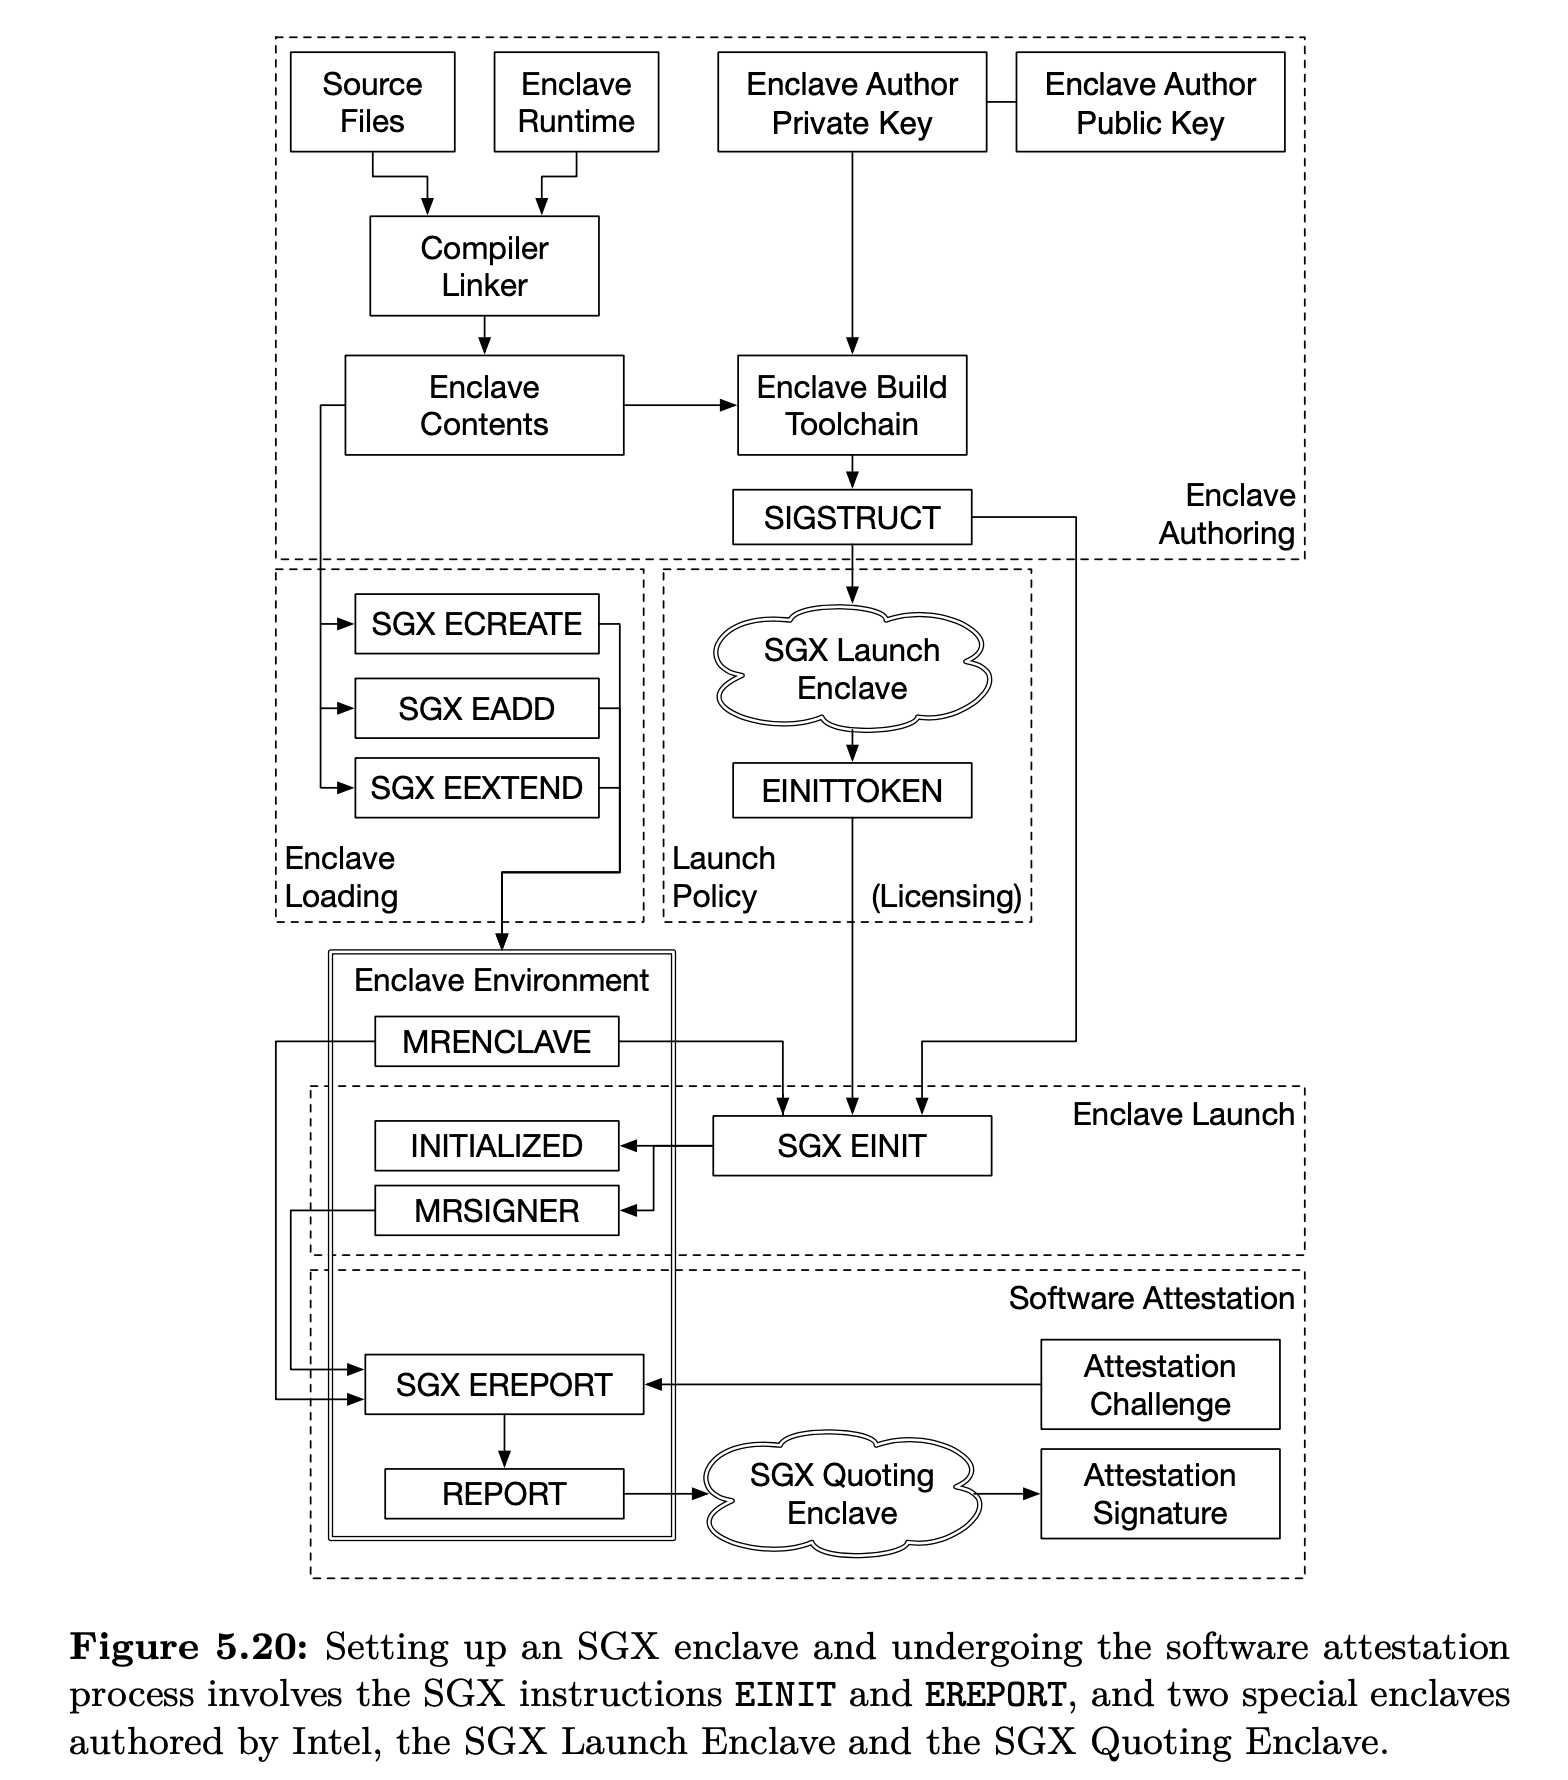
\includegraphics[width=0.8\textwidth]{images/SGX_software_attestation.png}
\caption{SGX 软件验证}
\label{SGXSoftwareAttestation}
\end{figure}

\subsubsection{本地验证}
飞地通过图\ref{EREPORT_data_flow}展示的EPEPORT指令向其他目标飞地发送自己的身份。EREPORT指令提供i个验证报告(REPORT),报告以加密方式将飞地提供的消息与飞地的基于度量和基于证书的身份绑定在一起。加密绑定是通过使用对称密钥计算的MAC标签完成的,该对称密钥仅在目标飞地和SGX实现之间共享。

\begin{figure}
\centering
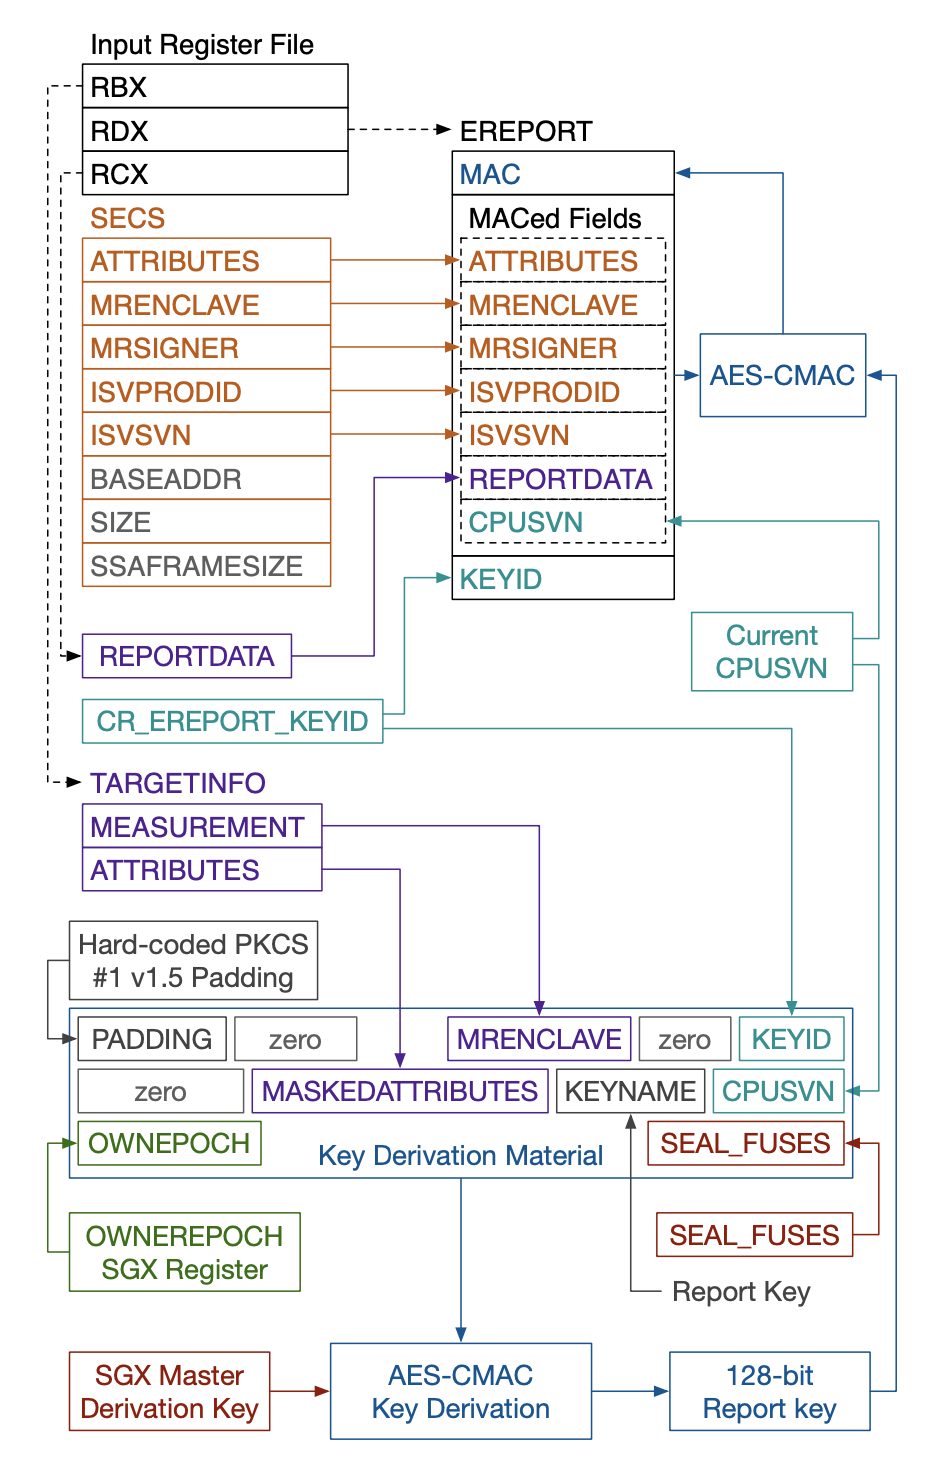
\includegraphics[width=0.8\textwidth]{images/EREPORT_data_flow.png}
\caption{EREPORT 数据流图}
\label{EREPORT_data_flow}
\end{figure}

EREPORT指令读取从飞地的SECS中当前飞地的身份信息,利用身份信息填充REPORT结构。具体来说


\subsection{}
